\subsection{Клиент}
Проектирование пользовательской части включает в себя разработку развёрнутой диаграммы классов, которая отражает взаимодействие между внутренними частями клиента, в частности графической оболочкой и классом, реализующим внутренний интерфейс. Также необходимо рассмотреть пользовательский интерфейс. Диаграмма классов должна быть отображена с точки зрения реализации, а не концептуальной позиции, как было в первой части работы.

Диаграмма классов (Class diagram)~-- статическая структурная диаграмма, описывающая структуру системы. Она демонстрирует классы системы, их атрибуты, методы и зависимости между классами.

\begin{figure}[ht]
\centering
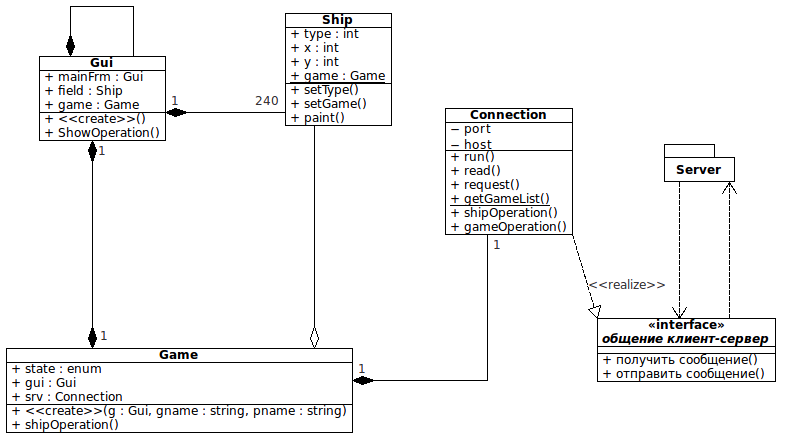
\includegraphics[width=18cm]{images/class_client.png}
\caption{Диаграмма классов клиента}
\label{fig8}
\end{figure}


Анализ правил и условий игры показал, что, для упрощения реализации, необходимо выделить класс Ship. Он должен отвечать за отображение кораблей на игровом поле, а так же за порядок действий остальных классов при нажатии на корабль.
Класс Game будет являться прослойкой между внутренним и графическим интерфейсами. Он описывает последовательности действий графической оболочки и отдельных кораблей, которые зависят от полученной команды Сервера. Примером такого взаимодействия является создание новой игры, описание которого представлено на рисунке [\ref{fig9}].

\begin{figure}[pt]
\centering
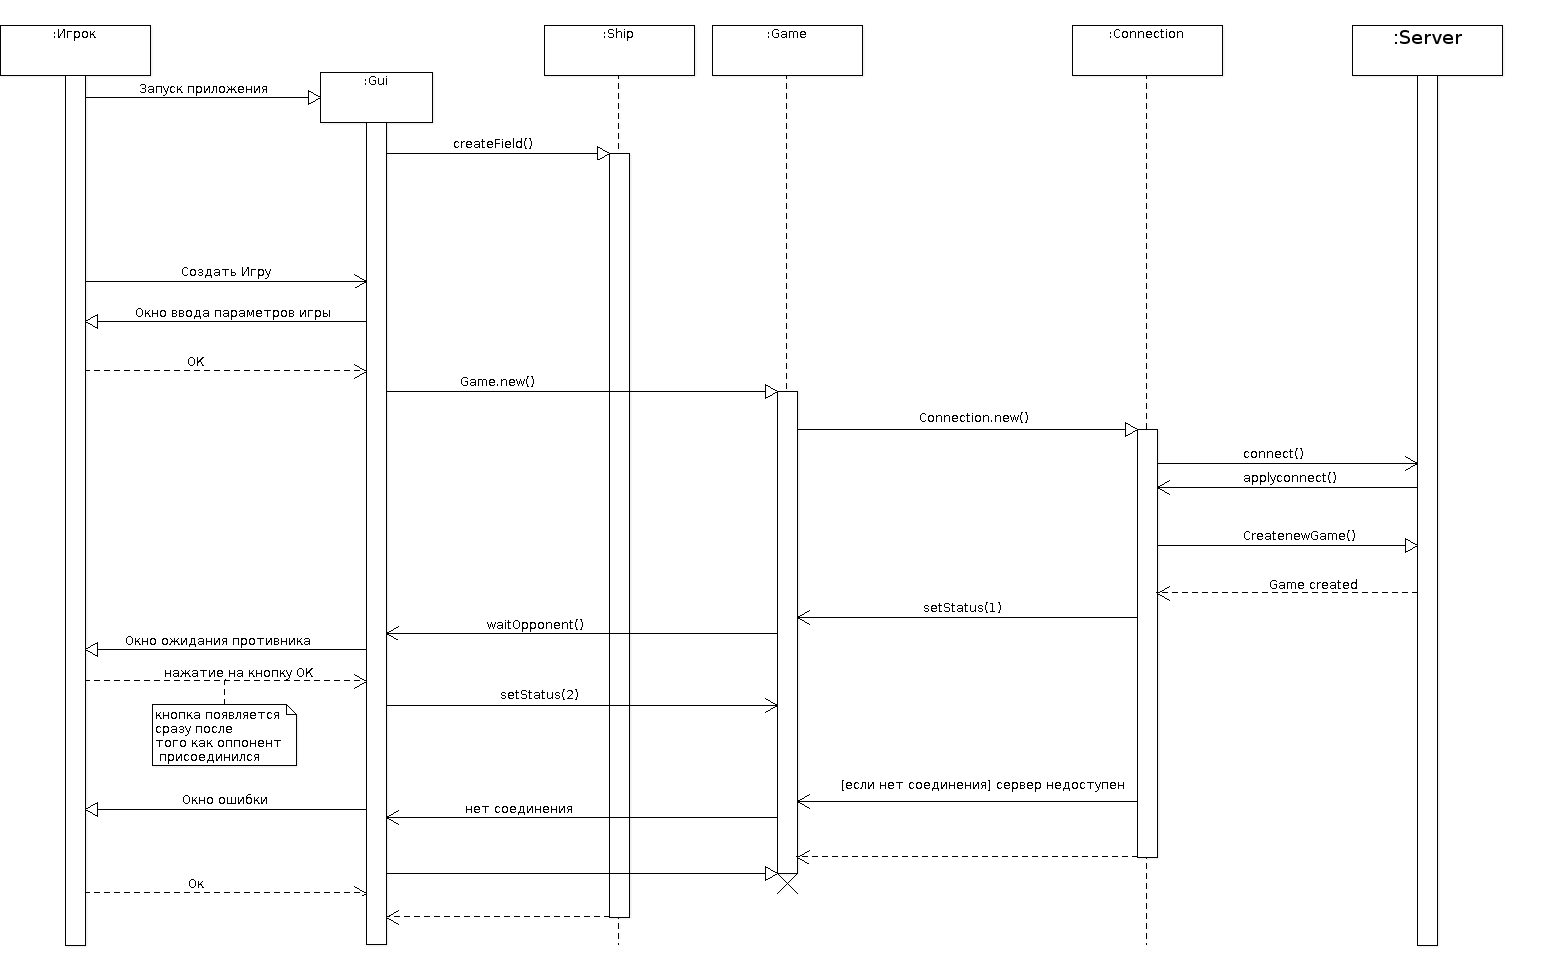
\includegraphics[width=15cm]{images/CRG.png}
\caption{Диаграмма создания новой игры}
\label{fig9}
\end{figure}


Ещё один аспект, который был включен на диаграмме [\ref{fig0}] в вариант использования <<Управление игрой>>,~-- это присоединение к игре, созданной другим игроком. Взаимодействие классов между собой при этом прецеденте показано на схеме [\ref{fig10}].

\begin{figure}[pt]
\centering
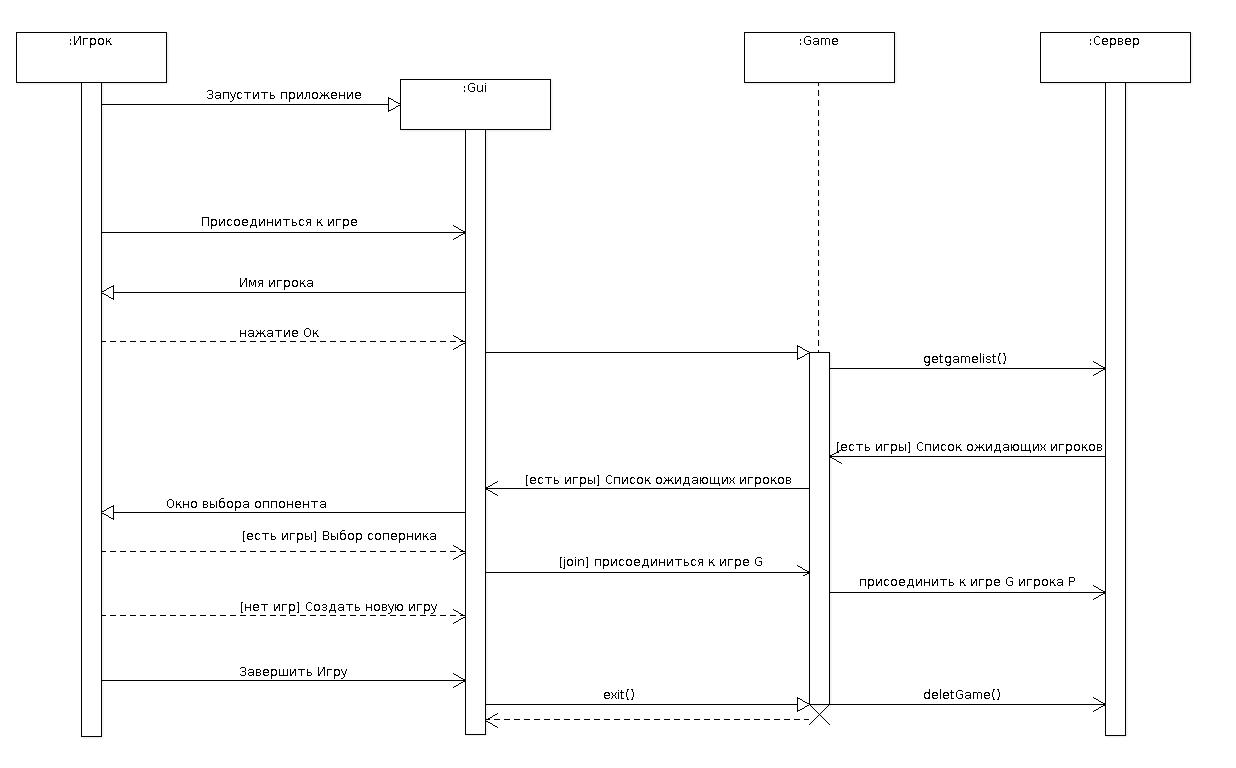
\includegraphics[width=15cm]{images/JG.png}
\caption{Диаграмма присоединения к игре}
\label{fig10}
\end{figure}

Действия, производимые над объектом класса Ship в течение всего процесса игры:
	\begin{itemize}
		\item Расстановка кораблей перед боем;
		\item Передвижение корабля;
		\item Атака корабля противника;
		\item Ответ на вопрос корабля противника;
		\item Взрыв бомбы;
		\item Взрыв торпеды;
  	\end{itemize} 
Естественно не все эти варианты следует отображать на диаграммах, так как многие из них сводятся к реализации простейших функций и не требуют детального проектирования. 
Расстановка кораблей, части которой можно использовать не только при формировании начального игрового поля, но и при описании процесса снятия и передвижения кораблей во время боя  приведена на диаграмме [\ref{fig11}].

\begin{figure}[pt]
\centering
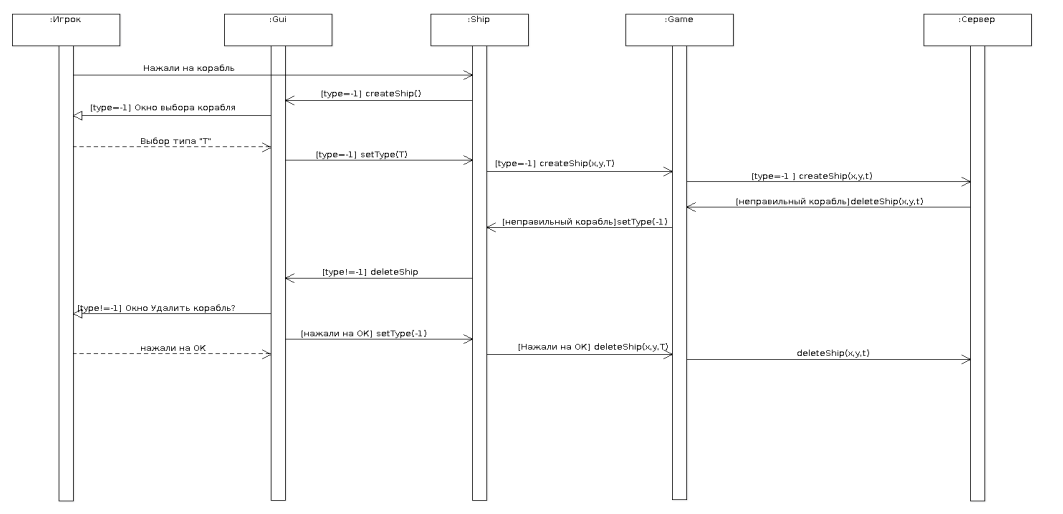
\includegraphics[width=12cm]{images/CRS.png}
\caption{Диаграмма установки корябля}
\label{fig11}
\end{figure}

Игра проходит в несколько этапов, от которых зависят возможности действий игроков. Зависимость между ними и действиями, которые предшествуют тому или иному состоянию, можно увидеть на диаграмме [\ref{fig12}].

\begin{figure}[ht]
\centering
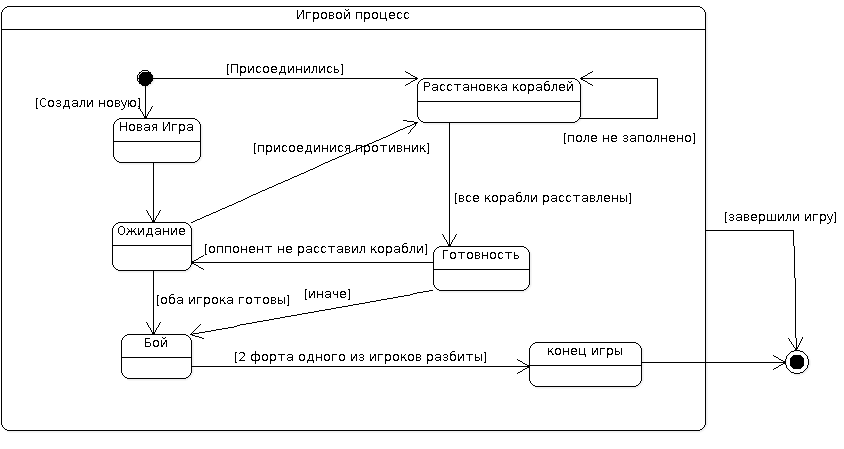
\includegraphics[width=18cm]{images/statecl.png}
\caption{Диаграмма состояний игры}
\label{fig12}
\end{figure}


Следует подчеркнуть, что состояние <<Бой>> на [\ref{fig12}] раскрыто не полностью, так как есть небольшие подсостояния, зависящие, к примеру, от очерёдности хода или совершаемого действия из списка возможных. Их можно выделять в отдельные состояния, которые будут рассмотрены в следующей части, так как относятся к правилам, контролируемым сервером. 
\endinput
